\documentclass[10pt]{article}
\pdfoutput=1%xelatex编译注释掉
\usepackage{../tex/NotesTeX}
\usepackage[UTF8]{ctex}  %pdfTex中文环境
\usepackage[utf8]{inputenc}  %调用\input函数
\usepackage{graphicx}  %图表环境
\usepackage{subfigure}	%并排图片宏%
\usepackage{booktabs}	%三线表线条
\usepackage{caption}	%可能要用到的图表标题宏包





%\usepackage{background}%封面背景
\usepackage{draftwatermark}  %水印,参数设置:仅在首页出现 [firstpage] ;仅在尾页出现 [lastpage]
\SetWatermarkText{DRAFT}  %水印自定义文字
%\SetWatermarkLightness{0.5}  %水印透明度,默认0.8,范围0-1
%\SetWatermarkScale{1}  %水印大小,默认1.2
%\usepackage{CTEX}  %xelatex编译中文环境



%\usepackage{showframe}
\title{\begin{center}{\Huge \textit{家用理论物理教程}}\\{{\itshape 从入门到转行}}\end{center}}
	\author{Shunz Dai\footnote{\href{https://ShunzDai.github.io/}{\textit{My Personal Blog}}}}
	
	
	\affiliation{
	Physics and Space Science College,China West Normal University
	}
	
	\emailAdd{196883@outlook.com}
	%\backgroundsetup{scale=1, angle=0, opacity = 0.1,contents = {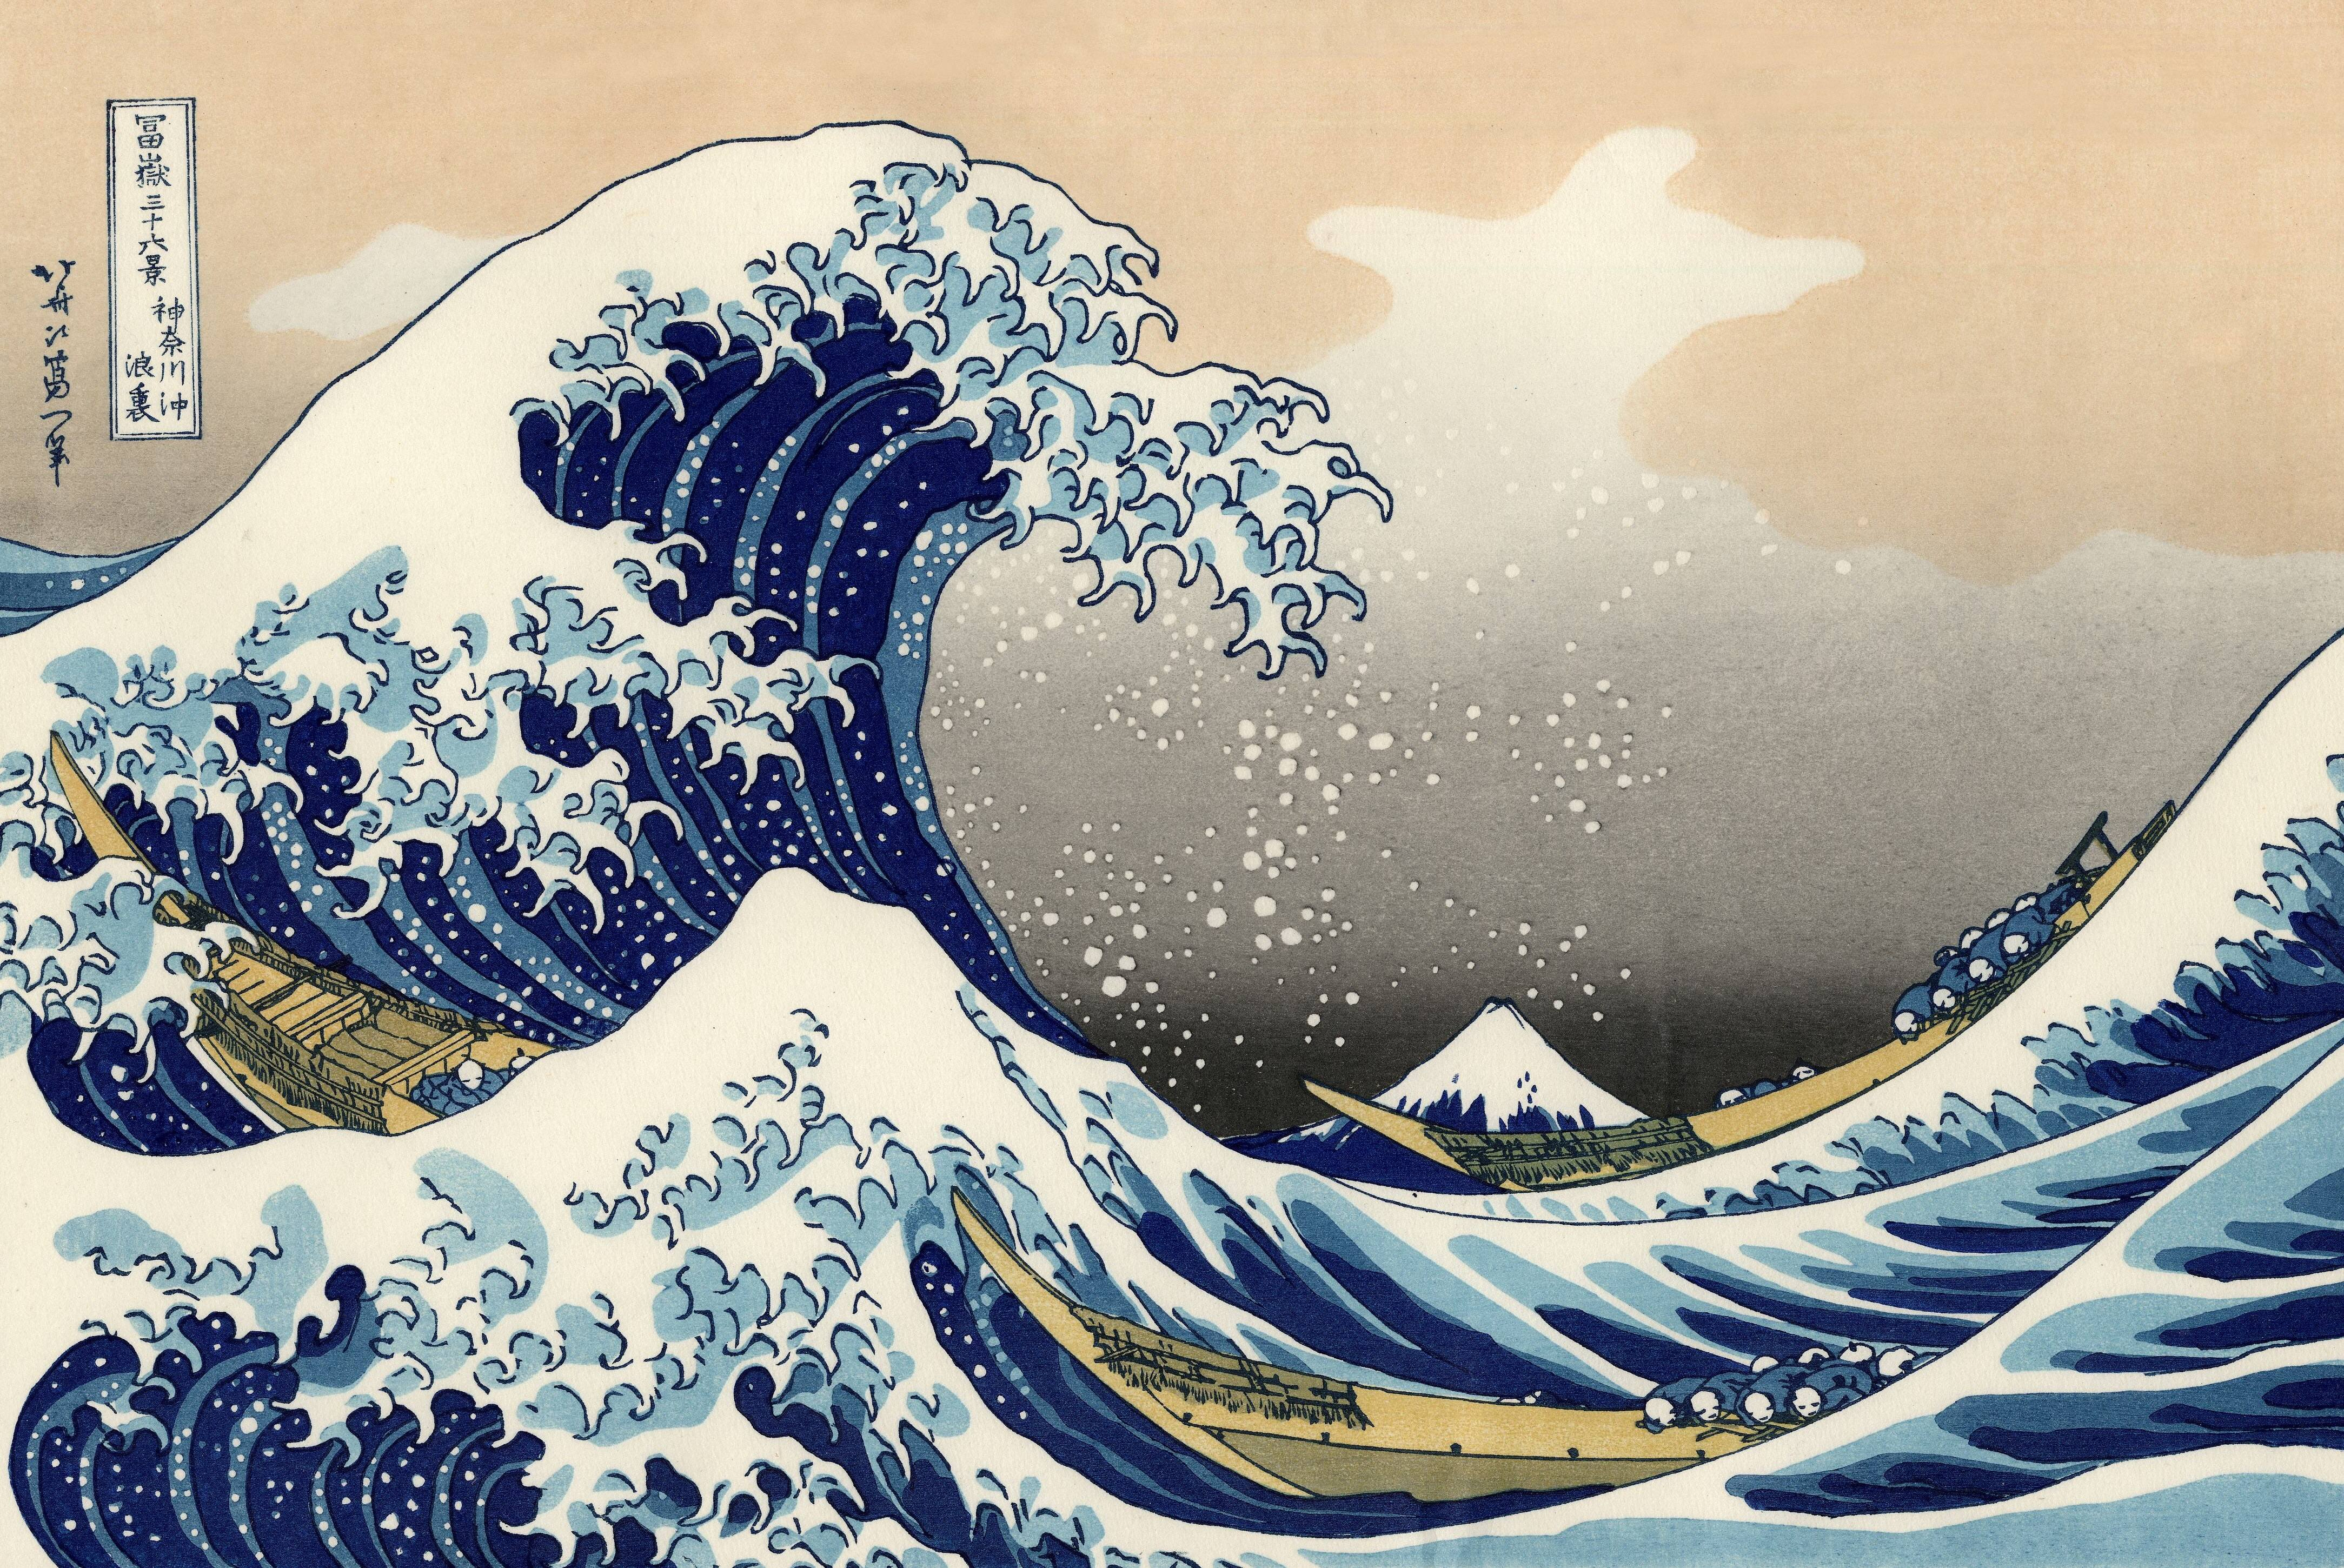
\includegraphics[width=\paperwidth, height=\paperwidth,keepaspectratio]{figures/background.png}}}
	
	
	\begin{document}
	
		\maketitle
		
		\flushbottom
		\newpage
		\pagestyle{fancynotes}
		\part{引言}
    我从2019年9月就开始写这份笔记了,但写到今天也只有寥寥数页。原本的笔记也有这样一个引言部分,主要讲述了我整个大学四年的艰难历程,但现在看来,那些文字只不过是自己感动自己罢了\footnote{我仍然保留了那些文字,放在我的博客中:\href{https://shunzdai.now.sh/2020/06/04/My-Life-In-College/}{\textit{我的大学}}。}。现在,我重写了这份引言,用尽量简短的语言来阐述这份笔记做了些什么工作。
	
    这份笔记受微分几何的影响颇深,微分几何也是我大学四年以来尤其喜爱的数学领域。相比于线性代数,微分几何为代数问题赋予了几何的看法;相比于微积分(当然,我指的是高等数学中的微积分,而不是数学分析中的微积分),微分几何更注重“基本结构”,它没有繁多的运算技巧,不必将问题拘谨在冗长的计算中。事实上,理论物理与微分几何的关系可以说是“殊途同归”,它们都用到了公理化(或者说是“第一性原理”)的方法。在研究这种问题时,我们总可以从几条基本公理(或基本假设)出发,逐步推理出宏伟的结构。
    
    在繁琐冗长的计算训练中,我们逐步忘却了那些基本结构的作用。当然,这些论断不意味着我们在学习理论物理时不需要任何实际计算、应用,只是说,我们在学习理论物理时更应该将注意力放在基本结构上,而简单的计算能够加深理解,这就已经足够了,我们不必将精力放在如同上述第一个问题的复杂计算上。

    这份笔记中,我们将通篇使用Einstein求和约定,即相同的一对上下指标表示求和。我们将始终保持上下指标的差异,这种差异原则上与度量张量升降指标无关,而是一种源自事物本身的“对偶”属性。

    希望诸位能喜欢上本教程。
    
    $\quad$

    $\quad$

    \rightline{代顺治}
    \rightline{2020年10月31日,于深圳}
    
		\part{微分几何}\label{Part:Differential_Geometry}
	\begin{margintable}\vspace{1.4in}\footnotesize
		\begin{tabularx}{\marginparwidth}{|X}
			
			%Section~\ref{sec:structure}. 张量场与微分形式场\\
			Section~\ref{sec:Riemannian_Manifold}. Riemannian流形\\
			
			%Section~\ref{sec:LieAlgebra}. 联络与曲率\\
		\end{tabularx}
	\end{margintable}
	我并不打算像通常的微分几何教程那样循规蹈矩,而是用一种我认为通俗易懂的描述构造non-Euclidean几何框架.当然,这样做会损失一些数学上的严谨性,但我认为这对于物理工作者而言无伤大雅.
	\section{切空间与余切空间}
		我们首先回顾一下线性空间的公理化定义.
		\begin{definition}
			域$F$上的线性空间$V$是这样一个集合,对任意$\alpha,\beta,\gamma\in V;a,b\in F$满足
			\begin{enumerate}
				矢量加法映射$V\times V\rightarrow V$:
				\item (交换律)$\alpha+\beta=\beta+\alpha$;
				\item (结合律)$(\alpha+\beta)+\gamma=\alpha+(\beta+\gamma)$;
				\item (零元)存在唯一的$0\in V$,使得$0+\alpha=\alpha$;
				\item (逆元)对任意$\alpha\in V$,存在唯一的$\beta\in V$,使得$\alpha+\beta=0$.
				
				矢量数乘映射$F\times V\rightarrow V$:
				\item (酉性)对$1\in F$,有$1\alpha=\alpha$;
				\item (结合律)$a(b\alpha)=(ab)\alpha$;
				\item (分配律1)$(a+b)\alpha=a\alpha+b\alpha$;
				\item (分配律2)$a(\alpha+\beta)=a\alpha+a\beta$.
			\end{enumerate}
		\end{definition}
		在第一次学习这个定义的时候,你可能会问:“这有什么意义?交换律,结合律,分配律,这些东西不是小学就学了么?”这就是公理化的奇妙之处.我们总是能从这样通俗易懂的基础逻辑出发,演绎出宏伟的结构.数学是这样,后面我们会看到理论物理(而不是材料物理)也是这样.
		
		一个最平凡的例子就是$n$维Euclidean空间$\mathbb{R}^n$.我们将$\mathbb{R}^n$中的元素称为\textbf{点},记为一个有序数组$(x^1,\cdots,x^n)$,或简记为$(x^\mu),\mu=1,\cdots,n$,其中$x^\mu$是$n$个称为\textbf{坐标}的实参数.容易证明$\mathbb{R}^n$完全满足线性空间的定义.
		
		事实上我们还可以引入不同的参数来表示空间中的同一点.例如,我们找来一组带撇的参数$x'^\mu$,然后将原来的$(x^1,\cdots,x^n)$转换为$(x'^1,\cdots,x'^n)$,这个过程称为\textbf{坐标变换},我们可以用一个映射$\varphi$表示之:
		\begin{equation}\label{eq:coordinate transformation}
			\varphi:\mathbb{R}^n\rightarrow \mathbb{R}^n,(x^1,\cdots,x^n)\Rightarrow(x'^1,\cdots,x'^n).
		\end{equation}
		我们注意到\ref{coordinate transformation}这个映射相当于“输入$(x^1,\cdots,x^n)$,得到$x'^1$;$\cdots$;输入$(x^1,\cdots,x^n)$,得到$x'^n$”,这就相当于$n$个$n$元函数:
		\begin{equation}
			\begin{split}
				\varphi^1&:\mathbb{R}^n\rightarrow \mathbb{R},(x^1,\cdots,x^n)\Rightarrow x'^1;\\
				&\cdots\\
				\varphi^n&:\mathbb{R}^n\rightarrow \mathbb{R},(x^1,\cdots,x^n)\Rightarrow x'^n.
			\end{split}
		\end{equation}
		这就是通常意义下的坐标变换函数组.
		\begin{margintable}\vspace{1.4in}\footnotesize
			\begin{tabularx}{\marginparwidth}{|X}
				
				%Section~\ref{sec:structure}. 张量场与微分形式场\\
				Section~\ref{sec:Riemannian_Manifold}. Riemannian流形\\
				
				%Section~\ref{sec:LieAlgebra}. 联络与曲率\\
			\end{tabularx}
		\end{margintable}	
		
		\begin{example}\ 
			
			\begin{enumerate}
				\item 直角坐标系
				
				  
			\end{enumerate}

		\end{example}
		现在,我们正式引入切空间.


		



	\section{张量场与微分形式场}


	\section{Riemannian流形}\label{sec:Riemannian_Manifold}
		一个流形指的是这样一个结构,其在局部上是平直的,但整体不必是平直的,为了描述这一属性,我们引入度规张量.


	\section{联络与曲率}
		对于任意标量场$\phi\in \varGamma(T_{(0,0)}M)$,其外微分$d\phi$仍是是一个张量场
		\begin{equation}
				 d\phi=\frac{\partial\phi}{\partial x^\mu}dx^\mu=\frac{\partial\phi}{\partial {x}^\mu}\frac{\partial{x}^\mu}{\partial {x'}^\nu}d{x'}^\nu=\frac{\partial{\phi'}}{\partial {x'}^\nu}d{x'}^\nu\in \varGamma(T_{(0,1)}M),
		\end{equation}
		这意味着$d\phi$仍是张量丛截面的元素,用学物理家的话来说也就是$d\phi$仍然满足张量的变换规律.
		
		一个自然的问题是,对于切矢量场或余切矢量场,其外微分是否仍然是张量丛截面的元素?但问题就出在这,外微分算子是一个定义在外形式丛截面上的线性算子,切矢量场不是外形式丛截面中的元素,因此我们无法对一个切矢量场求外微分;余切矢量场作为1微分形式场,虽然它是外形式丛截面的元素,但它只是一种全反对称的张量场,我们无法对一个一般的非全反对称张量场求外微分.这些困难意味着我们需要推广外微分算子,寻找一个定义在一般张量丛截面$\varGamma(T_{(p,q)}M)$上的线性微分算子,让我们能对那些不在外形式丛截面中的张量场进行“微分”运算.这样构造的线性微分算子就是\textbf{仿射联络}.
		\begin{remark}
		余切矢量场$\omega\in \varGamma(T_{(0,1)}M)$在局部坐标系改变时满足
		\begin{equation}\label{eq:domega1}
				\omega=\omega_\mu dx^\mu=\omega_\mu\frac{\partial{x}^\mu}{\partial {x'}^\nu}d{x'}^\nu=\omega'_\nu d{x'}^\nu,
		\end{equation}
		我们对(\ref{eq:domega1})求全微分得到
		\begin{eqnarray}\label{eq:domega2}
			d\omega &=&d\omega'_\nu{\wedge}d{x'}^\nu\notag\\
			&=&d\left(\omega_\mu\frac{\partial{x}^\mu}{{\partial}{x'}^\nu}\right)\wedge d{x'}^\nu\notag\\
			&=&\frac{\partial{x}^\mu}{{\partial}{x'}^\nu}d\omega_\mu{\wedge}d{x'}^\nu+\omega_{\mu}d\left(\frac{\partial{x}^\mu}{\partial {x'}^\nu}\right){\wedge}d{x'}^\nu\notag\\
			&=&\left(\frac{\partial{\omega}_\mu}{{\partial}{x}^\sigma}\frac{\partial{x}^\sigma}{\partial {x'}^\rho}\frac{\partial{x}^\mu}{{\partial}{x'}^\nu}+{\omega}_\mu\frac{\partial^2{x}^\mu}{\partial {x'}^\rho{\partial}{x'}^\nu}\right)d{x'}^\rho{\wedge}d{x'}^\nu\\
			&=&\frac{\partial\omega'_\nu}{{\partial}{x'}^\rho}d{x'}^\rho{\wedge}d{x'}^\nu\notag,
		\end{eqnarray}
		注意到\ref{eq:domega2}中产生了一个二阶偏微分项,与张量的变换规律对比可知,这一项破坏了张量的变换规律.但外微分形式场的全反对称特性可以消除掉这一项带来的影响,即
		\begin{eqnarray}
			\frac{\partial\omega'_\nu}{{\partial}{x'}^\rho}d{x'}^\rho{\wedge}d{x'}^\nu&=&2\partial'_{[\rho}\omega'_{\nu]}{dx'}^{\rho}\otimes{dx'}^\nu\notag\\
				&=&2\left(\partial_{[\sigma}\omega_{\mu]}\frac{\partial{x}^\sigma}{\partial {x'}^\rho}\frac{\partial{x}^\mu}{{\partial}{x'}^\nu}+{\omega}_\mu\frac{\partial^2{x}^\mu}{\partial {x'}^{[\rho}{\partial}{x'}^{\nu]}}\right){dx'}^{\rho}\otimes{dx'}^\nu\notag\\
			&=&2\partial_{[\sigma}\omega_{\mu]}\frac{\partial{x}^\sigma}{\partial {x'}^\rho}\frac{\partial{x}^\mu}{{\partial}{x'}^\nu}{dx'}^{\rho}\otimes{dx'}^\nu,
		\end{eqnarray}
		所以$d\omega$实际上仍是张量场.但微分形式场说到底只是一种特殊的全反对称张量场,对于一般的张量场,我们无法通过张量场自身的对称性消除上述二阶偏微分项.
		\end{remark}

		现代微分几何中的联络指的是一般矢量丛上的联络.这一节我们先讨论切丛$T_{(1,0)}(M)$上的联络(称为\textbf{仿射联络}),然后逐步构造出张量丛$T_{(p,q)}(M)$上的联络.下面,我们直接给出仿射联络的定义.
		\begin{definition}
			仿射联络是一个映射
			\begin{equation*}
				D:\varGamma(T_{(1,0)}M)\rightarrow \varGamma(T_{(1,1)}M),
			\end{equation*}
			它满足下列条件:
			\begin{enumerate}
				\item 对任意的$A,B\in \varGamma(T_{(1,0)}M)$有 D(A+B)=D(A)+D(B);						
				\item 对任意的$A\in \varGamma(T_{(1,0)}M),\alpha\in \varGamma(T_{(0,0)}M)$有$D(\alpha A)=d\alpha\otimes A+\alpha D(A)$.
			\end{enumerate}
		\end{definition}
		局部上,联络由一组1微分形式给出.我们先来看自然标架场$\{\partial_\mu\}$的联络,命
		\begin{equation}
		D(\partial_\mu)=\omega^\rho_\mu \otimes\partial_\rho={\varGamma^\rho}_{\mu\nu}dx^\nu\otimes \partial_\rho,
		\end{equation} 
		其中$\omega^\rho_\mu={\varGamma^\rho}_{\mu\nu}dx^\nu$,${\varGamma^\rho}_{\mu\nu}$称为\textbf{联络系数},它是局部坐标系中的光滑函数.将$\omega^\rho_\mu$作为矩阵$\omega$第$\rho$行第$\mu$列的元素,这样构造的矩阵$\omega$称为\textbf{联络方阵}.可见,任意两个联络间的差异完全体现在联络方阵上.现在,我们来看联络的变换规律.在标架变换下,由联络的定义立即得到
		\begin{eqnarray}
			D(\partial'_\nu)&=&D\left(\frac{\partial{x^\mu}}{\partial{x'}^\nu}{\partial}_\mu\right)\notag\\
			&=&d\left(\frac{\partial{x^\mu}}{\partial{x'}^\nu}\right)\otimes{\partial}_\mu+\frac{\partial{x^\mu}}{\partial{x'}^\nu}D\left({\partial}_\mu\right)\notag\\
			&=&\left[d\left(\frac{\partial{x^\rho}}{\partial{x'}^\nu}\right)+\frac{\partial{x^\mu}}{\partial{x'}^\nu}\omega^\rho_\mu\right]\otimes{\partial}_\rho\notag\\
			&=&\left[d\left(\frac{\partial{x^\rho}}{\partial{x'}^\nu}\right)\frac{\partial{{x'}^\sigma}}{\partial{x^\rho}}+\frac{\partial{x^\mu}}{\partial{x'}^\nu}\omega^\rho_\mu\frac{\partial{{x'}^\sigma}}{\partial{x^\rho}}\right]\otimes\partial'_\sigma\notag\\
			&=&{\omega'}^\sigma_\nu\otimes\partial'_\sigma,
		\end{eqnarray}
		其中
		\begin{equation}\label{eq:connection}
		{\omega'}^\sigma_\nu=d\left(\frac{\partial{x^\rho}}{\partial{x'}^\nu}\right)\frac{\partial{{x'}^\sigma}}{\partial{x^\rho}}+\frac{\partial{x^\mu}}{\partial{x'}^\nu}\omega^\rho_\mu\frac{\partial{{x'}^\sigma}}{\partial{x^\rho}},
		\end{equation}
		这就是联络方阵在局部标架场改变时的变换公式.我们还可以进一步展开(\ref{eq:connection}),得到
		\begin{equation}
		{{\varGamma'}^\sigma}_{\nu\lambda}=\frac{\partial^2{x^\rho}}{\partial{x'}^\lambda\partial{x'}^\nu}\frac{\partial{{x'}^\sigma}}{\partial{x^\rho}}+{\varGamma^\rho}_{\mu\alpha}\frac{\partial{x^\mu}}{\partial{x'}^\nu}\frac{\partial{x}^\alpha}{\partial{x'}^\lambda}\frac{\partial{{x'}^\sigma}}{\partial{x^\rho}},
		\end{equation}
		这正是通常意义下的联络变换公式.可见联络系数${\varGamma^\rho}_{\mu\nu}$并不是一个张量,但引入它能使$D(\partial_\mu)$遵循张量的变换规律.
		
		稍作思考可以发现,若使用全反对称化的技巧,我们也能利用联络系数构造出一个张量.我们将在稍后给出具体讨论.

		切丛截面的联络在余切丛截面上诱导出一个联络(仍记为$D$),易看出它是从$\varGamma(T_{(0,1)}M)$到\\$\varGamma(T_{(0,2)}M)$的映射.
		现在现在我们来考察$\{\partial_\mu\}$的对偶标架$\{dx^\mu\}$的联络.$D(dx^\mu)$由下式确定
		$$d\left(\partial_\mu,dx^\nu\right)=\left(D(\partial_\mu),dx^\nu\right)+\left(\partial_\mu,D(dx^\nu)\right),$$
		我们设
		$$D(dx^\nu)={\omega^*}^\nu_\rho\otimes{dx}^\rho,$$
		于是
		$$\left(\partial_\mu,D(dx^\nu)\right)=\left(\partial_\mu,{\omega^*}^\nu_\rho\otimes{dx}^\rho\right)={\omega^*}^\nu_\rho\delta^\rho_\mu={\omega^*}^\nu_\mu.$$
		考虑到对偶标架满足
		$$\left(\partial_\mu,dx^\nu\right)=\delta^\nu_\mu,$$ 
		于是得到
		\begin{eqnarray}
			{\omega^*}^\nu_\mu&=&\left(\partial_\mu,D(dx^\nu)\right)=-\left(D(\partial_\mu),dx^\nu\right)\\
				&=&-\left(\omega^\rho_\mu\otimes\partial_\rho,dx^\nu\right)=-{\omega}^\rho_\mu\delta^\nu_\rho=-{\omega}^\nu_\mu,
		\end{eqnarray}
		即
		$D(dx^\nu)=-{\omega}^\nu_\rho\otimes{dx}^\rho$.
		至此,我们就能计算任意$A\in T_{(1,0)}(M)$与$B\in T_{(0,1)}(M)$的联络了.在局部坐标系下,我们有:			\begin{eqnarray}
			\begin{split}
				D(A)&=D(A^\mu\partial_\mu)\\
				&=dA^\mu\otimes\partial_\mu+A^{\mu}D(\partial_\mu)\\
				&=(\partial_{\rho}A^\mu+A^{\nu}{\varGamma^\mu}_{\nu\rho})dx^\rho{\otimes}\partial_\mu\\
				&=\nabla_{\rho}A^{\mu}dx^\rho{\otimes}\partial_\mu;
			\end{split}
		\end{eqnarray}
		\begin{eqnarray}
			\begin{split}
				D(B)&=D(B_{\mu}{dx}^\mu)\\
				&=dB_\mu\otimes{dx}^\mu+B_{\mu}D({dx}^\mu)\\
				&=(\partial_{\rho}B_\mu-B_\nu{\varGamma^\nu}_{\mu\rho})dx^\rho{\otimes}dx^\mu\\
				&=\nabla_{\rho}B_{\mu}dx^\rho{\otimes}dx^\mu,
			\end{split}
		\end{eqnarray}
		其中
		\begin{eqnarray}
			\nabla_{\rho}A^\mu&=&\partial_{\rho}A^\mu+A^{\nu}{\varGamma^\mu}_{\nu\rho};\\
				\nabla_{\rho}B_{\mu}&=&\partial_{\rho}B_\mu-B_\nu{\varGamma^\nu}_{\mu\rho}.
		\end{eqnarray}							
		这正是通常意义下的\textbf{协变导数}运算.由此可见,协变导数是一种依赖于局部坐标系的分量表述.用类似的方法,我们能得到$T_{(p,q)}(M)$上的诱导联络.
		\begin{definition}在一般张量丛$T_{(p,q)}M$上,由仿射联络诱导的联络是一个映射
			$$D:\varGamma(T_{(p,q)}M)\rightarrow\varGamma(T_{(p,q+1)}M),$$
			设任意$S\in \varGamma(T_{(p,q)}M)$,则$S$的联络在局部坐标系下满足
			\begin{equation}
				\begin{split}
					D(S)&=D({S^{\mu_1\dots\mu_p}}_{\nu_1\dots\nu_q}\partial_{\mu_1}\otimes\dots\otimes\partial_{\mu_p}\otimes{dx}^{\nu_1}\otimes\dots\otimes{dx}^{\nu_q})\\
				%&=d({S^{\mu_1\dots\mu_p}}_{\nu_1\dots\nu_q})\otimes\partial_{\mu_1}\otimes\dots\otimes\partial_{\mu_p}\otimes{dx}^{\nu_1}\otimes\dots\otimes{dx}^{\nu_q}\notag\\
				%&+{S^{\mu_1\dots\mu_p}}_{\nu_1\dots\nu_q}D(\partial_{\mu_1})\otimes\dots\otimes\partial_{\mu_p}\otimes{dx}^{\nu_1}\otimes\dots\otimes{dx}^{\nu_q}\notag\\
				%&+\dots+{S^{\mu_1\dots\mu_p}}_{\nu_1\dots\nu_q}\partial_{\mu_1}\otimes\dots\otimes D({\partial_{\mu_p}})\otimes{dx}^{\nu_1}\otimes\dots\otimes{dx}^{\nu_q}\notag\\
				%&+{S^{\mu_1\dots\mu_p}}_{\nu_1\dots\nu_q}\partial_{\mu_1}\otimes\dots\otimes{\partial_{\mu_p}}\otimes D({dx}^{\nu_1})\otimes\dots\otimes{dx}^{\nu_q}\notag\\
				%&+\dots+{S^{\mu_1\dots\mu_p}}_{\nu_1\dots\nu_q}\partial_{\mu_1}\otimes\dots\otimes{\partial_{\mu_p}}\otimes{dx}^{\nu_1}\otimes\dots\otimes D({dx}^{\nu_q})\notag\\
				%&=(\partial_\rho{S^{\mu_1\dots\mu_p}}_{\nu_1\dots\nu_q}+{S^{\sigma\dots\mu_p}}_{\nu_1\dots\nu_q}{\varGamma^{\mu_1}}_{\sigma\rho}\notag\\
				%&+\dots+{S^{\mu_1\dots\sigma}}_{\nu_1\dots\nu_q}{\varGamma^{\mu_p}}_{\sigma\rho}-{S^{\mu_1\dots\mu_p}}_{\sigma\dots\nu_q}{\varGamma^{\sigma}}_{\nu_1\rho}\notag\\
				%&-\dots-{S^{\mu_1\dots\mu_p}}_{\nu_1\dots\sigma}{\varGamma^{\sigma}}_{\nu_q\rho})dx^\rho\otimes\partial_{\mu_1}\otimes\dots\otimes\partial_{\mu_p}\otimes{dx}^{\nu_1}\otimes\dots\otimes{dx}^{\nu_q}\notag\\
				&=\nabla_{\rho}{S^{\mu_1\dots\mu_p}}_{\nu_1\dots\nu_q}dx^\rho\otimes\partial_{\mu_1}\otimes\dots\otimes\partial_{\mu_p}\otimes{dx}^{\nu_1}\otimes\dots\otimes{dx}^{\nu_q},
				\end{split}
			\end{equation}
			其中
			\begin{equation}
				\begin{split}
					\nabla_{\rho}{S^{\mu_1\dots\mu_p}}_{\nu_1\dots\nu_q}&=\partial_\rho{S^{\mu_1\dots\mu_p}}_{\nu_1\dots\nu_q}\\
					&+{S^{\sigma\dots\mu_p}}_{\nu_1\dots\nu_q}{\varGamma^{\mu_1}}_{\sigma\rho}+\dots+{S^{\mu_1\dots\sigma}}_{\nu_1\dots\nu_q}{\varGamma^{\mu_p}}_{\sigma\rho}\\
					&-{S^{\mu_1\dots\mu_p}}_{\sigma\dots\nu_q}{\varGamma^{\sigma}}_{\nu_1\rho}-\dots-{S^{\mu_1\dots\mu_p}}_{\nu_1\dots\sigma}{\varGamma^{\sigma}}_{\nu_q\rho}.
				\end{split}		
			\end{equation}
		\end{definition}


\newpage
	
	
	
		
		\part{分析力学}\label{Part:Analytical}
	\begin{margintable}\vspace{1.4in}\footnotesize
		\begin{tabularx}{\marginparwidth}{|X}
			Section~\ref{sec:Lagrange}. Lagrange力学\\
			Section~\ref{sec:Hamilton}. Hamilton力学\\
		\end{tabularx}
	\end{margintable}

	在Newton力学体系中,我们用Newton方程研究力学系统的演化.所谓“Newton方程”指的是Newton第二定律
	\begin{equation}\label{eq:f=ma}
		\overrightarrow{F} =m\overrightarrow{a}=\frac{d\overrightarrow{p}}{dt},
	\end{equation}
	我们可以像下面这样修改(\ref{eq:f=ma})得到一个有意思的表述形式.我们假设系统所受的合外力是一个保守力,即对于任意一个有界闭区域$S$,$\overrightarrow{F}$满足
	\begin{equation}\label{eq:intfx}
		\int _{\partial S}F_\mu dx^\mu=0,
	\end{equation}
	其中$F_\mu$是$\overrightarrow{F}$在坐标系下的分量.对于任意保守力,我们可以引入一个标量场$V(x)$,使得$F_\mu=-\partial_\mu V(x)$.通过分析量纲可知,标量场$V(x)$应具有能量的量纲,我们将这个标量场称为\textbf{势场}.
	\begin{remark}
		对(\ref{eq:intfx})用一下Stokes定理可以得到\footnote{如果你对这里出现的符号并不熟悉,你可以选择直接跳过,这不会影响后续阅读.}
		$$0=\int_{\partial S}F_\mu dx^\mu=\int_S \partial_\nu F_\mu dx^\nu\wedge dx^\mu=-\int_S\partial_\nu \partial_\mu V(x) dx^\nu\wedge dx^\mu,$$
		可见引入标量场$V(x)$并不改变保守力$\overrightarrow{F}$的性质.
	\end{remark}
	于是,借助标量场$V(x)$我们可以将(\ref{eq:f=ma})改写为
	\begin{equation}\label{eq:eloriginal}
		-\partial_\mu V(x)-\frac{dp_\mu}{dt}=0.
	\end{equation}
	至此,我们的准备工作就差不多了.但你可能认为,将Newton方程从(\ref{eq:f=ma})变到(\ref{eq:eloriginal})好像并没有什么,怎么就“有意思”了?确实是这样,但我们要知道这只是一个开始,我们将在后面看到(\ref{eq:eloriginal})蕴含的优越性.
	%我们注意到(\ref{eq:intfx})中的$\overrightarrow{F}\cdot \overrightarrow{dx}$是一个标量,并且它具有能量的量纲\footnote{读者可以思考一下:为什么这里要强调一个“标量”具有能量的量纲?答案在下一页的侧边栏里.}.于是我们就知道了(\ref{eq:intfx})的含义是“质点围绕闭合路径运动一周时,保守力不会改变质点的机械能”.但我们说(\ref{eq:intfx})这个表述太“物理”了,例如,我可以问:$\overrightarrow{dx}$是什么?是有向线段吗?那有向线段又是什么?是矢量吗?如果是矢量,那它又是哪个线性空间里的矢量?……这些问题并不好回答.我的做法是将$\overrightarrow{F}\cdot \overrightarrow{dx}$
	\section{Lagrange力学}\label{sec:Lagrange}
		
		我们总是看到如“水自发的往低处流”,“光线的传播路径总是用时最少的路径”,或者“各种原子的核外电子排布总使得原子总能量最低”等观测现象.这种现象与数学中的“极值”概念相似,于是我们给出这样一个第一性原理,称为\textbf{最小作用量原理}.
		\begin{definition}
			客体的作用量取极值时,总能导出客体所满足的运动方程.
		\end{definition}
		这个定义云里雾里,什么是作用量?为什么作用量要取极值?我们给出这样的解释.
		
		作用量是这样一个无量纲的泛函
		\begin{equation}\label{eq:action1}
			S=\int ds,
		\end{equation}
		其中$ds$是某个微分式\footnote{$ds$本质上是一个微分形式场,即流形外形式丛的截面.我们这里只讨论$ds$是1微分形式场的情况,即普通的微分式.}.我们可以根据不同的情况分别考虑(\ref{eq:action1})的具体形式.令
		\begin{equation}\label{eq:action2}
			S=\int ds=\frac{1}{\alpha}\int L(x(t),\cdots,y(t);\dot{x}(t),\cdots,\dot{y}(t))dt,
		\end{equation}
		其中$\alpha$是一个比例系数,$L(x(t),\cdots,y(t);\dot{x}(t),\cdots,\dot{y}(t))$是一个函数,$t$是一个参数,这就是一般情形下的作用量.我们可以为式中的比例系数、函数以及参数赋予物理意义,使其拥有表征物理量的量纲,这样我们就可以使作用量描述物理系统了.例如,当我们设比例系数$\alpha$具有长度的量纲,将函数$L$解释为折射率$L=n(x)$,并将参数$t$诠释为光走的几何路程$t=l$,此时(\ref{eq:action2})就变成了
		$$S=\int ds=\frac{1}{\alpha}\int n(x)dl,$$
		这样构造的作用量描述的就是光程.等等.

		于是我们就解释了什么是作用量.现在,我们回答第二个问题,为什么作用量要取极值?很遗憾的是,我无法回答这个问题.最小作用量原理是一个第一性原理,它无法被证伪.但我们知道,物理学是一门以实验为基础的学科.我们用最小作用量原理可以导出各种系统的运动方程,而这些运动方程预言的物理现象经受住了大量实验的考验.凭借“证有不证无”的观念,如果要证明最小作用量原理是错的,就要求我们拿出一个不满足最小作用量原理预言的实验证据,我们可以拿这一实验证据去证明最小作用量原理的错误,但在此之前,我们将全盘接受这一原理.

		我们求作用量的极值时要使用\textbf{变分}.变分的运算规则几乎与微分完全一致,差异仅在作用对象上:前者作用在泛函上,后者作用在普通函数上.现在我们举一个利用最小作用量原理解决实际问题的例子,顺便看看变分是怎样运算的.
		\begin{example}
			(最速降线问题)求质点的轨迹方程,使得在同一平面上,质点由A点至B点用时最短.
			
			设质点轨迹方程为隐函数$$f(x(t),y(t))=0,$$其中$x$表示质点在水平方向上的坐标,$y$表示质点在竖直方向上的坐标,参数$t$表示时间.在一个无穷小的时间间隔$dt$内,质点将会移动
			\begin{eqnarray*}
				dl=\sqrt{(dx)^2+(dy)^2}=\sqrt{(dx)^2+\left(\frac{dy}{dx}\right)^2(dx)^2}=\sqrt{1+y'^2}dx,
			\end{eqnarray*}
			其中$y'\equiv dy/dx$.考虑到机械能守恒
			\begin{eqnarray*}
				\frac{1}{2}m\left(\frac{dl}{dt}\right)^2=mgy,
			\end{eqnarray*}
			于是我们得到质点的瞬时速度满足
			\begin{eqnarray*}
				\frac{dl}{dt}=\sqrt{2gy}=\frac{\sqrt{1+y'^2}}{dt}dx,
			\end{eqnarray*}
			即
			\begin{eqnarray*}
				dt=\sqrt{\frac{1+y'^2}{2gy}}dx.
			\end{eqnarray*}
			于是我们以$x$为参数,以$y,y'$为泛函变量构造作用量
			\begin{eqnarray*}
				S(y(x);y'(x))=\frac{1}{\alpha}\int^B_Adt=\frac{1}{\alpha}\int^B_A\sqrt{\frac{1+y'^2}{2gy}}dx,
			\end{eqnarray*}
			其中比例系数$\alpha$是一个具有时间量纲的常数.
		\end{example}
		
		

	\section{Hamilton力学}\label{sec:Hamilton}
		Lagrange力学描述的是位形流形上的力学规律,是比Newton力学更深刻的分析工具.然而,Lagrange力学也有不足:Euler-Lagrange方程是一个二阶方程,它在大多数情况下不易求解.如果能想办法让描述力学系统的方程的阶数降下来,则在求解运动规律时就方便多了.Hamilton力学由此而生.Hamilton力学是辛流形上的力学规律,其参数为广义坐标$x^\mu$以及广义动量$p_\mu$.Lagrange力学中有Lagrange函数$L(x^\mu;{\dot{x}}^\mu)$,对应的,Hamilton力学中也有Hamilton函数,我们将其表示为$H(x^\mu;p_\mu)$.由Hamilton函数逐步搭建的力学体系能提供丰富的信息,事实上,由Heisenberg建立的矩阵力学就来源于经典Hamilton力学的量子化.
	\subsection{Hamilton方程}
		对Lagrange函数$L(x^\mu;{\dot{x}}^\mu)$变分,得到
		\begin{equation}\label{eq:delta L}
		\delta L=\frac{\partial L}{\partial x^\mu}\delta x^\mu+\frac{\partial L}{\partial {\dot{x}}^\mu}\delta {\dot{x}}^\mu,
		\end{equation}
		Lagrange函数具有能量的量纲,于是Lagrange函数对广义速度的偏导数具有动量的量纲.不妨将这个具有动量量纲的量称为“广义动量”.
		\begin{definition}
		广义动量$p_\mu$定义为
		\begin{equation}
			p_\mu:=\frac{\partial L}{\partial {\dot{x}}^\mu}.
		\end{equation}
		\end{definition}
		于是(\ref{eq:delta L})可以改写成
		\begin{equation}\label{eq:delta L'}
		\delta L=\frac{\partial L}{\partial x^\mu}\delta x^\mu+p_\mu\delta {\dot{x}}^\mu;
		\end{equation}
		再根据Euler-Lagrange方程得到
		\begin{equation*}
		\frac{\partial L}{\partial x^\mu}=\frac{d}{dt}\frac{\partial L}{\partial {\dot{x}}^\mu}={\dot{p}}_\mu,
		\end{equation*}
		所以(\ref{eq:delta L'})变成
		\begin{equation}\label{eq:delta L''}
		\delta L={\dot{p}}_\mu\delta x^\mu+p_\mu\delta {\dot{x}}^\mu.
		\end{equation}
		为了得到某个以$p_\mu$为变量的变分,我们对(\ref{eq:delta L''})进行Legendre变换得到
		\begin{equation*}
		\delta L={\dot{p}}_\mu\delta x^\mu+\delta(p_\mu{\dot{x}}^\mu)-{\dot{x}}^\mu\delta p_\mu,
		\end{equation*}
		移项得到
		\begin{equation}\label{eq:delta H}
		\delta(p_\mu{\dot{x}}^\mu-L)=-{\dot{p}}_\mu\delta x^\mu+{\dot{x}}^\mu\delta p_\mu.
		\end{equation}
		所以,若
		\begin{definition}
		定义Hamilton函数为
		\begin{equation}
			H:=p_\mu{\dot{x}}^\mu-L,
		\end{equation}
		\end{definition}
		则$H$就是以$x^\mu$和$p_\mu$为变量的函数.于是我们可以建立如下原理
		\begin{theorem}
		Hamilton方程组是指如下两个方程
		\begin{equation}
			\begin{split}\label{eq:H}
				\frac{\partial H}{\partial x^\mu}&=-{\dot{p}}_\mu;\\
				\frac{\partial H}{\partial p_\mu}&={\dot{x}}^\mu.
			\end{split}
		\end{equation}
		\end{theorem}
		可见,Hamilton力学研究的是1阶方程,但方程的数量比Lagrange力学增加了一倍.
	
	\subsection{Poisson括号}
		设任意力学量$A$是$x^\mu$与$p_\mu$的函数$A(x^\mu(t);p_\mu(t))$,我们来研究$A$随时间变化的规律.由于
		\begin{equation}\label{eq:Poisson}
		\frac{dA}{dt}=\frac{\partial A}{\partial x^\mu}\frac{d x^\mu}{dt}+\frac{\partial A}{\partial p_\mu}\frac{dp_\mu}{dt},
		\end{equation}
		考虑到Hamilton方程(\ref{eq:H}),带入(\ref{eq:Poisson})得到
		\begin{equation}\label{eq:Poisson'}
		\frac{dA}{dt}=\frac{\partial A}{\partial x^\mu}\frac{\partial H}{\partial p_\mu}-\frac{\partial H}{\partial x^\mu}\frac{\partial A}{\partial p_\mu}.
		\end{equation}
		(\ref{eq:Poisson'})存在着一种反对称性,我们可以用一个双线性映射表示之.
		\begin{definition}
		以$x^\mu$与$p_\mu$为变量的力学量$X$与$Y$的Poisson括号为
		\begin{equation}\label{eq:PB}
			\{X,Y\}:=\frac{\partial X}{\partial x^\mu}\frac{\partial Y}{\partial p_\mu}-\frac{\partial Y}{\partial x^\mu}\frac{\partial X}{\partial p_\mu}.
		\end{equation}
		\end{definition}
		\begin{remark}
			Poisson括号满足
			\begin{enumerate}
				\item 反对称性:$\{X,Y\}=-\{Y,X\}$;
				\item Jacobi恒等式:$\{\{X,Y\},Z\}+\{\{Z,X\}Y\}+\{\{Y,Z\},X\}=0$.
			\end{enumerate}
			事实上Poisson括号构成一个\textbf{Lie代数},我们将在\ref{sec:LieAlgebra}中进一步论述Lie代数的性质.
		\end{remark}
		
		(\ref{eq:Poisson'})可用Poisson括号表示为
		\begin{equation}\label{eq:heq1}
		\frac{dA}{dt}=\{A,H\}.
		\end{equation}
		Hamilton方程也可以修改成Poisson括号的形式
		\begin{equation}
		\begin{split}
			\{p_\mu,H\}&={\dot{p}_\mu};\\
			\{x^\mu,H\}&={\dot{x}}^\mu,
		\end{split}
		\end{equation}
		而$x^\mu$和$p_\mu$的Poisson括号为
		\begin{equation}\label{eq:xp}
		\{x^\mu,p_\nu\}=\frac{\partial x^\mu}{\partial x^\rho}\frac{\partial p_\nu}{\partial p_\rho}-\frac{\partial p_\nu}{\partial x^\rho}\frac{\partial x^\mu}{\partial p_\rho}=\delta^\mu_\rho\delta^\rho_\nu=\delta^\mu_\nu,
		\end{equation}
		广义坐标、广义动量与自身的Poisson括号为
		\begin{eqnarray}\label{eq:xxpp}
			\{x^\mu,x^\nu\}&=&\frac{\partial x^\mu}{\partial x^\rho}\frac{\partial x^\nu}{\partial p_\rho}-\frac{\partial x^\nu}{\partial x^\rho}\frac{\partial x^\mu}{\partial p_\rho}=0;\\
			\{p_\mu,p_\nu\}&=&\frac{\partial p_\mu}{\partial x^\rho}\frac{\partial p_\nu}{\partial p_\rho}-\frac{\partial p_\nu}{\partial x^\rho}\frac{\partial p_\mu}{\partial p_\rho}=0.
		\end{eqnarray}

		回到$A$随时间变化的规律问题上,我们得到如下引理.
		\begin{lemma}
		若力学量$A(x^\mu;p_\mu)$与Hamiltonian的Poisson括号为零,即
		\begin{equation}
			\{A,H\}=0,
		\end{equation}
		则物理量$A$是一个\textbf{守恒荷}.
		\end{lemma}
		一个适当的例子能帮助我们理解守恒荷的物理意义.
		\begin{example}
		设局部坐标下某自由粒子的Lagrangian为
		$$L=\frac{1}{2}g_{\mu\nu}\dot{x}^\mu\dot{x}^\nu,$$
		则广义动量
		\begin{eqnarray*}
			p_\rho&&=\frac{\partial L}{\partial {\dot{x}}^\rho}=\frac{1}{2}g_{\mu\nu}\left(\frac{\partial \dot{x}^\mu}{\partial {\dot{x}}^\rho}\dot{x}^\nu+\dot{x}^\mu\frac{\partial \dot{x}^\nu}{\partial {\dot{x}}^\rho}\right)\\
			&&=\frac{1}{2}g_{\mu\nu}\left(\delta^\mu_\rho\dot{x}^\nu+\dot{x}^\mu\delta^\nu_\rho\right)=g_{\rho\mu}\dot{x}^\mu.
		\end{eqnarray*}
		因此$\dot{x}^\mu\equiv g^{\mu\nu}p_\nu$,于是Hamiltonian为
		\begin{eqnarray*}
			H=p_\mu{\dot{x}}^\mu-L=g^{\mu\nu}p_\mu p_\nu-\frac{1}{2}g^{\mu\nu}p_\mu p_\nu=\frac{1}{2}g^{\mu\nu}p_\mu p_\nu	
		\end{eqnarray*}
		用Poisson括号可得
		\begin{eqnarray*}
			\{p_\mu,H\}=0;\\
			\{H,H\}=0.
		\end{eqnarray*}	
		所以此时广义动量和Hamiltonian守恒.
		\end{example}
	
		Poisson括号构成了一个函数空间上的Lie代数,事实上,Poisson括号被量子化后就得到了对易括号,对易括号是某个算子空间上的Lie代数.Poisson括号与对易括号之间有如下对应法则
		\begin{equation}
		\{A,B\}\rightarrow\frac{1}{i\hbar}[\hat{A},\hat{B}],
		\end{equation}
		其中$[\hat{A},\hat{B}]:=\hat{A}\hat{B}-\hat{B}\hat{A}$.
	
	\subsection{Noether定理}
		\begin{theorem}
		设$\epsilon$是一个无穷小量.若无穷小坐标变换$x^\mu\rightarrow x'^\mu=x^\mu+\epsilon f^\mu(x)$保持Hamiltonian不变,则$Q\equiv p_\mu f^\mu(x)$是一个守恒荷.
		\end{theorem}
		\begin{proof}
		要证$Q$是守恒荷,即证$\dot{Q}$为零:
		\begin{equation*}
			\begin{split}
				\dot{Q}&\equiv\frac{dQ}{dt}=\{Q,H\}\\
				&=\frac{\partial Q}{\partial x^\rho}\frac{\partial H}{\partial p_\rho}-\frac{\partial H}{\partial x^\rho}\frac{\partial Q}{\partial p_\rho}\\
				&=p_\mu \frac{\partial f^\mu}{\partial x^\rho}\frac{\partial H}{\partial p_\rho}-f^\rho\frac{\partial H}{\partial x^\rho}.
			\end{split}
		\end{equation*}
		下面来计算Hamiltonian的变分.由于坐标变换保持Hamiltonian不变,则有$\delta H=0$,于是
		\begin{equation}\label{pr:delta H}
			0=\delta H=\frac{\partial H}{\partial x^\mu}\delta x^\mu+\frac{\partial H}{\partial p_\mu}\delta p_\mu,
		\end{equation}
		其中$\delta x^\mu$可直接由坐标变换得到:
		\begin{equation}\label{pr:delta x}
			\begin{split}
				x^\mu\rightarrow x'^\mu&=x^\mu+\epsilon f^\mu(x)\\
				\Rightarrow\delta x^\mu&=\epsilon f^\mu(x);
			\end{split}
		\end{equation}
		$\delta p_\mu$要从广义动量的定义出发得到:
		\begin{eqnarray*}
			&&p_\mu=\frac{\partial L}{\partial \dot{x}^\mu}\\
			\Rightarrow &&p'_\mu=\frac{\partial L}{\partial \dot{x}'^\mu}=\frac{\partial L}{\partial \dot{x}^\nu}\frac{\partial \dot{x}^\nu}{\partial \dot{x}'^\mu}=p_\nu\frac{\partial \dot{x}^\nu}{\partial \dot{x}'^\mu},
		\end{eqnarray*}
		由坐标变换可推得
		\begin{eqnarray*}
			&&x'^\mu=x^\mu+\epsilon f^\mu(x)\\
			\Rightarrow&&\dot{x}'^\mu=\dot{x}^\mu+\epsilon \frac{\partial f^\mu}{\partial x^\rho}\dot{x}^\rho\\
			\Rightarrow&&\frac{\partial \dot{x}'^\mu}{\partial \dot{x}^\nu}=\delta^\mu_\nu+\epsilon \frac{\partial f^\mu}{\partial x^\rho}\delta^\rho_\nu=\delta^\mu_\nu+\epsilon \frac{\partial f^\mu}{\partial x^\nu}\\
			\Rightarrow&&\frac{\partial \dot{x}^\nu}{\partial \dot{x}'^\mu}=\delta^\nu_\mu-\epsilon \frac{\partial f^\nu}{\partial x^\mu},
		\end{eqnarray*}
		其中最后一步可用反证法证明
		\begin{eqnarray*}
			\frac{\partial \dot{x}'^\mu}{\partial \dot{x}^\nu}\frac{\partial \dot{x}^\nu}{\partial \dot{x}'^\rho}=\left(\delta^\mu_\nu+\epsilon \frac{\partial f^\mu}{\partial x^\nu}\right)\left(\delta^\nu_\mu-\epsilon \frac{\partial f^\nu}{\partial x^\mu}\right)=\delta^\mu_\rho+O(\epsilon^2),
		\end{eqnarray*}
		省略高阶无穷小只剩单位矩阵,说明左侧两个矩阵确实是互逆的.但我们尚未证明逆矩阵的唯一性,为此,我们假设
		\begin{eqnarray*}
			\frac{\partial \dot{x}^\nu}{\partial \dot{x}'^\mu}=\delta^\nu_\mu+\epsilon h^\nu_\mu,
		\end{eqnarray*}
		其中$h^\nu_\mu$是以坐标为变量的函数.于是
		\begin{eqnarray*}
			\delta^\mu_\rho&&=\frac{\partial \dot{x}'^\mu}{\partial \dot{x}^\nu}\frac{\partial \dot{x}^\nu}{\partial \dot{x}'^\rho}\\
			&&=\left(\delta^\mu_\nu+\epsilon \frac{\partial f^\mu}{\partial x^\nu}\right)\left(\delta^\nu_\rho+\epsilon h^\nu_\rho\right)\\
			&&=\delta^\mu_\rho+\epsilon\left(\frac{\partial f^\mu}{\partial x^\rho}+h^\mu_\rho\right)+O(\epsilon^2)\\
			&&\Rightarrow\epsilon\left(\frac{\partial f^\mu}{\partial x^\rho}+h^\mu_\rho\right)=0,
		\end{eqnarray*}
		要使上式对于任意无穷小量$\epsilon$都成立,唯有	
		\begin{eqnarray*}
			h^\mu_\rho=-\frac{\partial f^\mu}{\partial x^\rho},
		\end{eqnarray*}
		这样就证明了解的唯一性.所以
		\begin{equation}\label{pr:delta p}
		\begin{split}
			p'_\mu&=p_\nu\frac{\partial \dot{x}^\nu}{\partial \dot{x}'^\mu}=p_\nu\left(\delta^\nu_\mu-\epsilon \frac{\partial f^\nu}{\partial x^\mu}\right)\\
			&=p_\mu-\epsilon p_\nu\frac{\partial f^\nu}{\partial x^\mu}\\
			\Rightarrow\delta p_\mu&=-\epsilon p_\nu\frac{\partial f^\nu}{\partial x^\mu}
		\end{split}
		\end{equation}	
		将(\ref{pr:delta x})和(\ref{pr:delta p})带入(\ref{pr:delta H})得到
		\begin{equation}\label{pr:delta H'}
		\begin{split}
			0=\delta H&=-\epsilon\left[p_\nu\frac{\partial f^\nu}{\partial x^\mu}\frac{\partial H}{\partial p_\mu}-f^\mu\frac{\partial H}{\partial x^\mu}\right]=-\epsilon\dot{Q}.
		\end{split}
		\end{equation}
		要使(\ref{pr:delta H'})对于任意的无穷小量$\epsilon$都成立,唯有$\dot{Q}=0$,得证.\\
		\end{proof}
	
		\begin{theorem}
		守恒荷$Q$是无穷小坐标变换的生成元.
		\end{theorem}
	
		力学量$A(x^\mu;p_\mu)$的变分为
		\begin{eqnarray*}
		\delta A=\frac{\partial A}{\partial x^\mu}\delta x^\mu+\frac{\partial A}{\partial p_\mu}\delta p_\mu,
		\end{eqnarray*}
		从上面对守恒荷的证明可知,$\delta x^\mu$和$\delta p_\mu$能够借助守恒荷$Q$表述为
		\begin{exercise}
			\begin{equation}\label{eq:generator}
				\begin{split}
					\delta x^\mu&=\epsilon f^\mu=\epsilon\{x^\mu,Q\};\\
					\delta p_\mu&=-\epsilon p_\nu\frac{\partial f^\nu}{\partial x^\mu}=\epsilon\{p_\mu,Q\}.
				\end{split}
			\end{equation}
		\end{exercise}
		
		(\ref{eq:generator})请读者自行证明.因此$\delta A$可以进一步写成
		\begin{eqnarray*}
		\delta A=\epsilon\left(\frac{\partial A}{\partial x^\mu}\{x^\mu,Q\}+\frac{\partial A}{\partial p_\mu}\{p_\mu,Q\}\right).
		\end{eqnarray*}
		在经典情形下,生成元构造尚不明显.但在Poisson括号量子化后,可以非常明显的展示出生成元构造.例如
		\begin{eqnarray*}
		x^\mu\rightarrow x'^\mu&&=x^\mu+\delta x^\mu\\
		&&=x^\mu+\epsilon[x^\mu,Q]\\
		&&=x^\mu-\epsilon Qx^\mu+\epsilon x^\mu Q\\
		&&=\left(1-\epsilon Q\right)x^\mu\left(1+\epsilon Q\right)\\
		&&=e^{-\epsilon Q}x^\mu e^{\epsilon Q},
		\end{eqnarray*}
		其中第四个等号省略了$O(\epsilon^2)$.
	\newpage
		\part{广义相对论}\label{Part:GR}
	\section{微分几何}\label{sec:DG}
		\begin{margintable}\vspace{1.4in}\footnotesize
			\begin{tabularx}{\marginparwidth}{|X}
			Section~\ref{sec:DG}. 微分几何\\
			Section~\ref{sec:structure}. 结构数学\\
			Section~\ref{sec:LieAlgebra}. Lie代数\\
			\end{tabularx}
		\end{margintable}
	\subsection{微分流形}
	
	
	\subsection{张量场与微分形式场}
	
	
	\subsection{联络与曲率}
		对于任意标量场$\phi\in T_{(0,0)}(M)$,其外微分是一个张量场
		\begin{equation}
			\begin{split}
				 d\phi=\frac{\partial\phi}{\partial x^\mu}dx^\mu=\frac{\partial\phi}{\partial {x}^\mu}\frac{\partial{x}^\mu}{\partial {x'}^\nu}d{x'}^\nu=\frac{\partial{\phi'}}{\partial {x'}^\nu}d{x'}^\nu.
			\end{split}
		\end{equation}
		这是说,一个自然的问题是:对于切矢量场或余切矢量场,其外微分是否仍然是张量场?我们以余切矢量场为例,计算其外微分在坐标变换下的性质.
		
		对于一个余切矢量场$\omega\in T_{(0,1)}(M)$,借助局部坐标系可将其表述为
		\begin{equation}\label{eq:domega}
			\begin{split}
				\omega=\omega_\mu dx^\mu=\omega_\mu\frac{\partial{x}^\mu}{\partial {x'}^\nu}d{x'}^\nu=\omega'_\nu d{x'}^\nu,
			\end{split}
		\end{equation}
		\ref{eq:domega}的全微分在坐标变换下满足
		\begin{equation}
			\begin{split}	
			d\omega &=d\omega'_\nu{\wedge}d{x'}^\nu\\
			&= d\left(\omega_\mu\frac{\partial{x}^\mu}{{\partial}{x'}^\nu}\right)\wedge d{x'}^\nu\\
			&=\frac{\partial{x}^\mu}{{\partial}{x'}^\nu}d\omega_\mu{\wedge}d{x'}^\nu+\omega_{\mu}d\left(\frac{\partial{x}^\mu}{\partial {x'}^\nu}\right){\wedge}d{x'}^\nu\\
			&=\left(\frac{\partial{\omega}_\mu}{{\partial}{x}^\sigma}\frac{\partial{x}^\sigma}{\partial {x'}^\rho}\frac{\partial{x}^\mu}{{\partial}{x'}^\nu}+{\omega}_\mu\frac{\partial^2{x}^\mu}{\partial {x'}^\rho{\partial}{x'}^\nu}\right)d{x'}^\rho{\wedge}d{x'}^\nu\\
			&=\frac{\partial\omega'_\nu}{{\partial}{x'}^\rho}d{x'}^\rho{\wedge}d{x'}^\nu.
			\end{split}
		\end{equation}
		注意到过程中产生了一个二阶偏微分项,与张量的变换规律对比可知,这一项破坏了张量的变换规律.但外代数的全反对称特性可以消除掉这一项带来的影响,即
		\begin{equation}
			\begin{split}
				\frac{\partial\omega'_\nu}{{\partial}{x'}^\rho}d{x'}^\rho{\wedge}d{x'}^\nu&=2\partial'_{[\rho}\omega'_{\nu]}{dx'}^{\rho}\otimes{dx'}^\nu\\
				&=2\left(\partial_{[\sigma}\omega_{\mu]}\frac{\partial{x}^\sigma}{\partial {x'}^\rho}\frac{\partial{x}^\mu}{{\partial}{x'}^\nu}+{\omega}_\mu\frac{\partial^2{x}^\mu}{\partial {x'}^{[\rho}{\partial}{x'}^{\nu]}}\right){dx'}^{\rho}\otimes{dx'}^\nu\\
			&=2\partial_{[\sigma}\omega_{\mu]}\frac{\partial{x}^\sigma}{\partial {x'}^\rho}\frac{\partial{x}^\mu}{{\partial}{x'}^\nu}{dx'}^{\rho}\otimes{dx'}^\nu,
			\end{split}
		\end{equation}
		所以$d\omega$实际上仍是张量场。但微分形式场说到底只是一种特殊的张量场。对于一般的张量场,我们无法通过张量场自身的全反对称性消除上述二阶偏微分项。并且,我们也没有定义过切矢量场的外微分。这些困难意味着外微分运算不能直接推广到张量空间$T_{(p,q)}(M)$上去,于是,我们希望构造出一种定义在张量空间上的新的微分运算,使得任意张量场在这种微分运算下满足张量的变换规律。为此,我们引入\textbf{联络}。
	
		\subsubsection{仿射联络}
		现代微分几何中的联络指的是一般矢量丛上的联络.这一节我们先讨论切丛$T_{(1,0)}(M)$上的联络(称为\textbf{仿射联络}),然后逐步构造出张量丛$T_{(p,q)}(M)$上的联络.下面,我们直接给出仿射联络的定义.
		\begin{definition}
			仿射联络是一个映射
			\begin{equation*}
				D:T_{(1,0)}(M)\rightarrow T_{(1,1)}(M),
			\end{equation*}
			它满足下列条件:
			\begin{enumerate}
				\item 对任意的$A,B\in T_{(1,0)}(M)$有 D(A+B)=D(A)+D(B);						
				\item 对任意的$A\in T_{(1,0)}(M),\alpha\in T_{(0,0)}(M)$有$D(\alpha A)=d\alpha\otimes A+\alpha D(A)$.
			\end{enumerate}
		\end{definition}
		局部上,联络由一组1微分形式给出.我们先看自然标架场$\{\partial_\mu\}$的联络.命
		\begin{equation}
		D(\partial_\mu)=\omega^\rho_\mu \otimes\partial_\rho={\Gamma^\rho}_{\mu\nu}dx^\nu\otimes \partial_\rho,
		\end{equation} 
		其中$\omega^\rho_\mu={\Gamma^\rho}_{\mu\nu}dx^\nu$,${\Gamma^\rho}_{\mu\nu}$称为\textbf{联络系数},它是局部坐标系中的光滑函数.以$\omega^\rho_\mu$作为矩阵$\omega$第$\rho$行第$\mu$列的元素,这样构造的矩阵$\omega$称为\textbf{联络方阵}.可见,任意两个联络间的差异完全体现在联络方阵上.现在,我们来看联络的变换规律.在标架变换下,由联络的定义立即得到			 
		\begin{equation}
			\begin{split}
			D(\partial'_\nu) &= D\left(\frac{\partial{x^\mu}}{\partial{x'}^\nu}{\partial}_\mu\right) \\
			&= d\left(\frac{\partial{x^\mu}}{\partial{x'}^\nu}\right)\otimes{\partial}_\mu+\frac{\partial{x^\mu}}{\partial{x'}^\nu}D\left({\partial}_\mu\right)\\
			&= \left[d\left(\frac{\partial{x^\rho}}{\partial{x'}^\nu}\right)+\frac{\partial{x^\mu}}{\partial{x'}^\nu}\omega^\rho_\mu\right]\otimes{\partial}_\rho\\
			&= \left[d\left(\frac{\partial{x^\rho}}{\partial{x'}^\nu}\right)\frac{\partial{{x'}^\sigma}}{\partial{x^\rho}}+\frac{\partial{x^\mu}}{\partial{x'}^\nu}\omega^\rho_\mu\frac{\partial{{x'}^\sigma}}{\partial{x^\rho}}\right]\otimes\partial'_\sigma\\
			&={\omega'}^\sigma_\nu\otimes\partial'_\sigma,
			\end{split}
		\end{equation}
		其中
		\begin{equation}\label{eq:connection}
		{\omega'}^\sigma_\nu=d\left(\frac{\partial{x^\rho}}{\partial{x'}^\nu}\right)\frac{\partial{{x'}^\sigma}}{\partial{x^\rho}}+\frac{\partial{x^\mu}}{\partial{x'}^\nu}\omega^\rho_\mu\frac{\partial{{x'}^\sigma}}{\partial{x^\rho}},
		\end{equation}
		这就是联络方阵在局部标架场改变时的变换公式.我们还可以进一步展开\ref{eq:connection},得到
		\begin{equation}
		{{\Gamma'}^\sigma}_{\nu\lambda}=\frac{\partial^2{x^\rho}}{\partial{x'}^\lambda\partial{x'}^\nu}\frac{\partial{{x'}^\sigma}}{\partial{x^\rho}}+{\Gamma^\rho}_{\mu\alpha}\frac{\partial{x^\mu}}{\partial{x'}^\nu}\frac{\partial{x}^\alpha}{\partial{x'}^\lambda}\frac{\partial{{x'}^\sigma}}{\partial{x^\rho}},
		\end{equation}
		这正是通常意义下的联络变换公式.可见联络系数${\Gamma^\rho}_{\mu\nu}$并不是一个张量,但引入它能使$D(\partial_\mu)$遵循张量的变换规律.但稍作思考可以发现,若使用全反对称化的技巧,我们也能利用联络系数构造出一个张量.我们将在下一节给出具体讨论.
	
		切丛的联络在余切丛上诱导出一个联络(仍记为$D$),易看出它是从$T_{(0,1)}(M)$到$T_{(0,2)}(M)$的映射.
		\begin{remark}
			相比于外微分算子,可见余切丛上的诱导联络算子将值域从外形式丛的截面(元素即全反对称的张量场)扩展到了一般的张量丛的截面(元素即一般的张量场).所以我们说联络是外微分算子在一般张量丛上的推广.
		\end{remark}
		现在现在我们来考察$\{\partial_\mu\}$的对偶标架$\{dx^\mu\}$的联络.$D(dx^\mu)$由下式确定
		$$d\left(\partial_\mu,dx^\nu\right)=\left(D(\partial_\mu),dx^\nu\right)+\left(\partial_\mu,D(dx^\nu)\right),$$
		我们设
		$$D(dx^\nu)={\omega^*}^\nu_\rho\otimes{dx}^\rho,$$
		于是
		$$\left(\partial_\mu,D(dx^\nu)\right)=\left(\partial_\mu,{\omega^*}^\nu_\rho\otimes{dx}^\rho\right)={\omega^*}^\nu_\rho\delta^\rho_\mu={\omega^*}^\nu_\mu.$$
		考虑到对偶标架满足
		$$\left(\partial_\mu,dx^\nu\right)=\delta^\nu_\mu,$$ 
		于是得到								 
		\begin{equation}
			\begin{split}
				{\omega^*}^\nu_\mu&=\left(\partial_\mu,D(dx^\nu)\right)=-\left(D(\partial_\mu),dx^\nu\right)\\
				&=-\left(\omega^\rho_\mu\otimes\partial_\rho,dx^\nu\right)=-{\omega}^\rho_\mu\delta^\nu_\rho=-{\omega}^\nu_\mu,
			\end{split}
		\end{equation}								 
		即
		$D(dx^\nu)=-{\omega}^\nu_\rho\otimes{dx}^\rho$.
		至此,我们就能计算任意$A\in T_{(1,0)}(M)$与$B\in T_{(0,1)}(M)$的联络了.借助局部坐标系,我们有:								 
		\begin{equation}
			\begin{split}
				D(A)&=D(A^\mu\partial_\mu)=dA^\mu\otimes\partial_\mu+A^{\mu}D(\partial_\mu)\\
				&=(\partial_{\rho}A^\mu+A^{\nu}{\Gamma^\mu}_{\nu\rho})dx^\rho{\otimes}\partial_\mu=\nabla_{\rho}A^{\mu}dx^\rho{\otimes}\partial_\mu;\\
				D(B)&=D(B_{\mu}{dx}^\mu)=dB_\mu\otimes{dx}^\mu+B_{\mu}D({dx}^\mu)\\
				&=(\partial_{\rho}B_\mu-B_\nu{\Gamma^\nu}_{\mu\rho})dx^\rho{\otimes}dx^\mu=\nabla_{\rho}B_{\mu}dx^\rho{\otimes}dx^\mu,
			\end{split}	
		\end{equation}
		其中									 
		\begin{equation}
			\begin{split}
				\nabla_{\rho}A^\mu&=\partial_{\rho}A^\mu+A^{\nu}{\Gamma^\mu}_{\nu\rho};\\
				\nabla_{\rho}B_{\mu}&=\partial_{\rho}B_\mu-B_\nu{\Gamma^\nu}_{\mu\rho}.
			\end{split}		
		\end{equation}								
		这正是通常意义下的\textbf{协变导数}运算.由此可见,协变导数是一种依赖于局部坐标系的分量表述.用类似的方法,我们能得到$T_{(p,q)}(M)$上的诱导联络.
		\begin{definition}
			$T_{(p,q)}(M)$
			设任意$S\in T_{(p,q)}(M)$,借助局部坐标系$\{x^\mu\}$,可将$S$的联络表述为
			\begin{equation}
				\begin{split}
					D(S)&=D({S^{\mu_1\dots\mu_p}}_{\nu_1\dots\nu_q}\partial_{\mu_1}\otimes\dots\otimes\partial_{\mu_p}\otimes{dx}^{\nu_1}\otimes\dots\otimes{dx}^{\nu_q})\\
					&=d({S^{\mu_1\dots\mu_p}}_{\nu_1\dots\nu_q})\otimes\partial_{\mu_1}\otimes\dots\otimes\partial_{\mu_p}\otimes{dx}^{\nu_1}\otimes\dots\otimes{dx}^{\nu_q}\\
					&+{S^{\mu_1\dots\mu_p}}_{\nu_1\dots\nu_q}D(\partial_{\mu_1})\otimes\dots\otimes\partial_{\mu_p}\otimes{dx}^{\nu_1}\otimes\dots\otimes{dx}^{\nu_q}\\
					&+\dots+{S^{\mu_1\dots\mu_p}}_{\nu_1\dots\nu_q}\partial_{\mu_1}\otimes\dots\otimes D({\partial_{\mu_p}})\otimes{dx}^{\nu_1}\otimes\dots\otimes{dx}^{\nu_q}\\
					&+{S^{\mu_1\dots\mu_p}}_{\nu_1\dots\nu_q}\partial_{\mu_1}\otimes\dots\otimes{\partial_{\mu_p}}\otimes D({dx}^{\nu_1})\otimes\dots\otimes{dx}^{\nu_q}\\
					&+\dots+{S^{\mu_1\dots\mu_p}}_{\nu_1\dots\nu_q}\partial_{\mu_1}\otimes\dots\otimes{\partial_{\mu_p}}\otimes{dx}^{\nu_1}\otimes\dots\otimes D({dx}^{\nu_q})\\
					&=(\partial_\rho{S^{\mu_1\dots\mu_p}}_{\nu_1\dots\nu_q}+{S^{\sigma\dots\mu_p}}_{\nu_1\dots\nu_q}{\Gamma^{\mu_1}}_{\sigma\rho}\\
					&+\dots+{S^{\mu_1\dots\sigma}}_{\nu_1\dots\nu_q}{\Gamma^{\mu_p}}_{\sigma\rho}-{S^{\mu_1\dots\mu_p}}_{\sigma\dots\nu_q}{\Gamma^{\sigma}}_{\nu_1\rho}\\
					&-\dots-{S^{\mu_1\dots\mu_p}}_{\nu_1\dots\sigma}{\Gamma^{\sigma}}_{\nu_q\rho})dx^\rho\otimes\partial_{\mu_1}\otimes\dots\otimes\partial_{\mu_p}\otimes{dx}^{\nu_1}\otimes\dots\otimes{dx}^{\nu_q}\\
					&=\nabla_{\rho}{S^{\mu_1\dots\mu_p}}_{\nu_1\dots\nu_q}dx^\rho\otimes\partial_{\mu_1}\otimes\dots\otimes\partial_{\mu_p}\otimes{dx}^{\nu_1}\otimes\dots\otimes{dx}^{\nu_q},
				\end{split}		
			\end{equation}
			其中
			\begin{equation}
				\begin{split}
					\nabla_{\rho}{S^{\mu_1\dots\mu_p}}_{\nu_1\dots\nu_q}&=\partial_\rho{S^{\mu_1\dots\mu_p}}_{\nu_1\dots\nu_q}+{S^{\sigma\dots\mu_p}}_{\nu_1\dots\nu_q}{\Gamma^{\mu_1}}_{\sigma\rho}\\
					&+\dots+{S^{\mu_1\dots\sigma}}_{\nu_1\dots\nu_q}{\Gamma^{\mu_p}}_{\sigma\rho}-{S^{\mu_1\dots\mu_p}}_{\sigma\dots\nu_q}{\Gamma^{\sigma}}_{\nu_1\rho}\\
					&-\dots-{S^{\mu_1\dots\mu_p}}_{\nu_1\dots\sigma}{\Gamma^{\sigma}}_{\nu_q\rho}.
				\end{split}		
			\end{equation}
		\end{definition}
	
	\newpage
		\part{量子场论}\label{Part:QFT}
	\begin{margintable}\vspace{1.4in}\footnotesize
		\begin{tabularx}{\marginparwidth}{|X}
		Section~\ref{sec:QM}. 量子力学\\
		\end{tabularx}
	\end{margintable}
	测试测试测试测试测试测试测试测试测试测试测试测试测试测试测试测试测试测试测试测试测试测试测试测试测试测试测试测试测试
	\section{量子力学}\label{sec:QM}
		
		笼统的说,将一个经典物理系统进行量子化的方法有三种.
		
		第一种方法是利用波动力学进行量子化,这种方法的核心是Schrodinger方程
		\begin{equation}
			-\frac{\hbar^2}{2m}\nabla^2\psi(\overrightarrow{x},t)+V(\overrightarrow{x})\psi(\overrightarrow{x},t)=i\hbar\frac{\partial}{\partial t}\psi(\overrightarrow{x},t).
		\end{equation}
		如你所见,Schrodinger方程是一个复的二阶偏微分方程,整个波动力学围绕这个方程展开,不停的解方程,这一过程用到的那些特殊函数我至今没有弄懂.但我可以不负责任的说,整个量子力学的核心不是微分方程,而是代数.因此,接下来的内容与你会不会球谐函数、Legendre函数无关紧要.

		第二种方法是利用矩阵力学进行量子化,这种方法来源于Hamilton力学.之前,我们在Hamilton力学中引入了一个Lie代数结构,称为Poisson括号.通过计算我们发现,整个Ha-
		milton力学都能改写成Poisson括号的形式,体现出和谐的统一性.使用这种方法,我们能对量子力学进行公理化构造,得出非常好的结论.

		至于第三种方法,我们先卖个关子,等到\ref{sec:#}再进行阐述.

		现在,我们给出量子力学的5条公理,接下来的内容完全建立在这5条公理之上.我们要声明,这5条公理不可证伪,因此不存在“为什么是这样”的问题.物理归根结底是一门以实验为基础的学科,以这5条公理为基础建立的整个量子力学体系经受了住大量实验的验证,因此我们说这5条公理是有效的.
		\begin{definition}
			给定一个孤立的力学系统,可根据如下5条公理构建一个量子力学系统:
			\begin{enumerate}
				\item 存在一个复Hilbert空间$\mathcal{H}$,量子系统的状态由$\mathcal{H}$中的矢量$\vert\psi\rangle$	描述,两个矢量$\vert\psi\rangle ,c\vert\psi\rangle(c\in\mathbb{C})$	描述相同状态.		
				\item 经典力学中的力学量$A(\overrightarrow{x} ,t)$对应了$\mathcal{H}$中的一个Hermitian算子
				$$\hat{A}(\overrightarrow{x} ,t):\mathcal{H}\rightarrow \mathcal{H},\hat{A}=\hat{A}^\dagger.$$
				对$A$的测量值是$\hat{A}$的特征值.
				\item 力学量$A,B$的Poisson括号对应了Hermitian算符$\hat{A},\hat{B}$的对易括号
				$$\{A,B\}\Rightarrow\frac{1}{i\hbar}[\hat{A},\hat{B}],$$
				其中$[\hat{A},\hat{B}]=\hat{A}\hat{B}-\hat{B}\hat{A}$.
				\item 若某一时刻量子系统处于$\vert\psi\rangle$状态,我们记此时测量力学量$A$的期望为$\langle A\rangle$,它满足
				$$\langle A\rangle =\frac{\langle\psi\vert\hat{A}\vert\psi\rangle}{\langle\psi\vert\psi\rangle}.$$
				\item 豆腐脑要吃甜的.
			\end{enumerate}
		\end{definition}
		\begin{remark}\ 
			\begin{enumerate}
				\item 完备的内积空间即Hilbert空间.其中完备性要求空间中的任意Cauchy序列均收敛,内积结构使得空间拥有了度量.
				
				$\mathcal{H}$存在一个对偶空间$\mathcal{H}^*$,$\mathcal{H}^*$中的矢量记为$\langle\psi\vert$.设算子$\hat{A}$的一组特征值$\{a_n\}$对应的正交归一特征向量为$\vert n\rangle $,满足$\langle m\vert n\rangle=\delta_{mn}$,其中由$\langle\cdot \vert\cdot\rangle:\mathcal{H}\times \mathcal{H}\rightarrow \mathbb{C} $诱导的内积结构就是$\mathcal{H}$上的内积.
				\item 算子$\hat{A}$的Hermitian性使得$\hat{A}$的特征值必定是实数.这是因为
				\begin{eqnarray*}
					\hat{A}\vert\psi_n\rangle=a_n\vert\psi_n\rangle&\Rightarrow&\langle\psi_n\vert\hat{A}\vert\psi_n\rangle=a_n\langle\psi_n\vert\psi_n\rangle;\\
					\langle\psi_n\vert\hat{A}^\dagger=a^*_n\langle\psi_n\vert&\Rightarrow&\langle\psi_n\vert\hat{A}^\dagger\vert\psi_n\rangle=a^*_n\langle\psi_n\vert\psi_n\rangle,
				\end{eqnarray*}
				考虑到$\hat{A}$的Hermitian性,于是有
				$$a^*_n\langle\psi_n\vert\psi_n\rangle=\langle\psi_n\vert\hat{A}^\dagger\vert\psi_n\rangle=\langle\psi_n\vert\hat{A}\vert\psi_n\rangle=a_n\langle\psi_n\vert\psi_n\rangle,$$
				即$a^*_n=a_n$.要使等式成立,则$a_n$必为实数.这样约定是因为量子系统中出现的测量值为复数时没有意义.
				\item 由(\ref{eq:xxppxp})得
				\begin{eqnarray*}
					\{x^\mu,x^\nu\}&=&0\Rightarrow\frac{1}{i\hbar}[\hat{x}^\mu,\hat{x}^\nu]=0;\\
					\{p_\mu,p_\nu\}&=&0\Rightarrow\frac{1}{i\hbar}[\hat{p}_\mu,\hat{p}_\nu]=0;\\
					\{x^\mu,p_\nu\}&=&\delta^\mu_\nu\Rightarrow\frac{1}{i\hbar}[\hat{x}^\mu,\hat{p}_\nu]=\delta^\mu_\nu.
				\end{eqnarray*}
				\item 若系统的状态矢量$\vert\psi\rangle$是归一化的,则$\langle\psi\vert\psi\rangle=1$,此时$\langle A\rangle =\langle\psi\vert\hat{A}\vert\psi\rangle$.
				\item 豆腐脑不可以是咸的.
			\end{enumerate}
		\end{remark}

		接下来我们便可以开始正题了.
		\subsection{绘景}
			首先,我们给出一个描述力学量算符随时间演化的方程,称为Heisenberg方程.
			\begin{definition}Heisenberg方程是对(\ref{eq:heq1})量子化的结果
				\begin{equation}\label{eq:heq2}
					\frac{dA}{dt}=\{A,H\}\Rightarrow\frac{d\hat{A}}{dt}=\frac{1}{i\hbar}[\hat{A},\hat{H}].
				\end{equation}
			\end{definition}
			(\ref{eq:heq2})是Hamilton力学在量子力学公理下的直接结论,它的解具有特别的结构.
			\begin{lemma}
				(\ref{eq:heq2})的解形如
				\begin{equation}\label{eq:heq'ssolution}
					\hat{A}(t)=e^{-\frac{1}{i\hbar}\hat{H}t}\hat{A}(0)e^{\frac{1}{i\hbar}\hat{H}t}.
				\end{equation}
				
			\end{lemma}
			\begin{proof}
				\begin{eqnarray*}
					\frac{d}{d t}\left(e^{-\frac{1}{i \hbar} \hat{H} t} \hat{A}(0) e^{\frac{1}{i \hbar} \hat{H} t}\right)&=&\frac{d}{d t}\left(e^{-\frac{1}{i \hbar}\hat{H} t}\right)\hat{A}(0) e^{\frac{1}{i \hbar} \hat{H} t}+e^{-\frac{1}{i \hbar} \hat{H} t} \hat{A}(0) \frac{d}{d t}\left(e^{\frac{1}{i \hbar} \hat{H} t}\right)\\
					&=&-\frac{1}{i \hbar} \hat{H} e^{-\frac{1}{i \hbar} \hat{H} t} \hat{A}(0) e^{\frac{1}{i \hbar} \hat{H} t}+e^{-\frac{1}{i \hbar} \hat{H} t} \hat{A}(0) \frac{1}{i \hbar} \hat{H} e^{\frac{1}{i \hbar} \hat{H} t} \\
					&=&-\frac{1}{i \hbar} \hat{H} \hat{A}(t)+\frac{1}{i \hbar} \hat{A}(t) \hat{H}=\frac{1}{i \hbar}[\hat{A}, \hat{H}].
				\end{eqnarray*}
			\end{proof}
			\begin{remark}
				为简化记号,我们命
			\begin{eqnarray*}
				U(t)&\equiv&e^{\frac{1}{i \hbar} \hat{H} t};\\
				U^\dagger (t)&\equiv&e^{-\frac{1}{i \hbar} \hat{H} t},
			\end{eqnarray*}
			于是(\ref{eq:heq'ssolution})可以写成
			\begin{equation}\label{eq:heq'ssolution2}
				\hat{A}(t)=U^\dagger(t)\hat{A}(0)U(t).
			\end{equation}
			\end{remark}
			
			我们将Heisenberg方程描述的体系称为Heisenberg绘景.在Heisenberg绘景下,算符含时,态不含时.我们设系统的归一化的状态为$\vert\psi\rangle_H$,则力学量$A(t)$的期望
			\begin{eqnarray}
				\langle A\rangle&=&\langle\psi\vert_H\hat{A}(t)\vert\psi\rangle_H\notag\\
				&=&\langle\psi\vert_H U^\dagger(t)\hat{A}(0)U(t)\vert\psi\rangle_H\notag\\
				&=&\langle\psi(t)\vert_S\hat{A}(0)\vert\psi(t)\rangle_S,
			\end{eqnarray}
			其中
			\begin{equation}\label{eq:transformation}
				\vert\psi(t)\rangle_S=U(t)\vert\psi\rangle_H,
			\end{equation}
			这个操作称为绘景变换——它将Heisenberg绘景下的状态矢量$\vert\psi\rangle_H$变换为Schrodinger绘景下的状态矢量$\vert\psi(t)\rangle_S$.在Schrodinger绘景下,算符不含时,态含时.我们将(\ref{eq:transformation})两侧同时对时间求导,于是得到
			\begin{equation}\label{eq:seq1}
				\frac{\partial}{\partial t}|\psi\rangle_{S}=\frac{\partial}{\partial t} e^{\frac{1}{i \hbar} \hat{H} t}|\psi\rangle_{H}=\frac{1}{i \hbar} \hat{H} e^{\frac{1}{i \hbar} \hat{H} t}|\psi\rangle_{H}=\frac{1}{i\hbar} \hat{H}|\psi\rangle_{S},
			\end{equation}
			(\ref{eq:seq1})即Schrodinger方程
			\begin{definition}Schrodinger方程为
				\begin{equation}\label{eq:seq2}
					\hat{H}|\psi\rangle_{S}=i\hbar\frac{\partial}{\partial t}|\psi\rangle_{S}.
				\end{equation}
			\end{definition}



\newpage
		\part{附录}\label{Part:Appendix}
	
	\begin{margintable}\vspace{1.4in}\footnotesize
		\begin{tabularx}{\marginparwidth}{|X}
		Section~\ref{sec:Dimensional}. 常见物理量的单位换算关系\\
		Section~\ref{sec:N_Sphere}. $n$维球的体积与表面积
		\end{tabularx}
	\end{margintable}

	


	


			
		
	\end{document}


	%\begin{equation}  公式居中编号
	%	\begin{split}
			
	%	\end{split}
	%\end{equation}

	%\notag  某行公式不编号